\section{Newton Expansion}

In continuous calculus, smooth functions can be expanded in a power
series called the Taylor series:

\[
f(x)
=
f(0)
+
f'(0)x
+
\frac{f''(0)}{2!}x^2
+
\frac{f^{(3)}(0)}{3!}x^3
+\cdots.
\]

Discrete calculus has a closely analogous expansion in terms of
falling factorials and finite differences.  This expansion is known as
the \emph{Newton expansion}.

\subsection*{Newton Expansion Theorem}

\begin{theorem}[Newton Expansion]
Let \(f : \mathbb{Z} \to \mathbb{R}\).  Then \(f\) can be expressed as

\[
f(x)
=
f(0)
+
\Delta f(0)\,x
+
\frac{\Delta^2 f(0)}{2!}\,x^{\underline{2}}
+
\frac{\Delta^3 f(0)}{3!}\,x^{\underline{3}}
+\cdots,
\]

where

\[
x^{\underline{k}} = x(x-1)(x-2)\cdots(x-k+1)
\]

denotes the falling factorial.
\end{theorem}

\subsection*{Interpretation}

The coefficients in this expansion are determined by the successive
finite differences of the function evaluated at \(0\):

\[
f(0),\quad
\Delta f(0),\quad
\Delta^2 f(0),\quad
\Delta^3 f(0),\dots
\]

These values appear naturally in the difference table of the function.

\subsection*{Difference Table Illustration}

\begin{center}
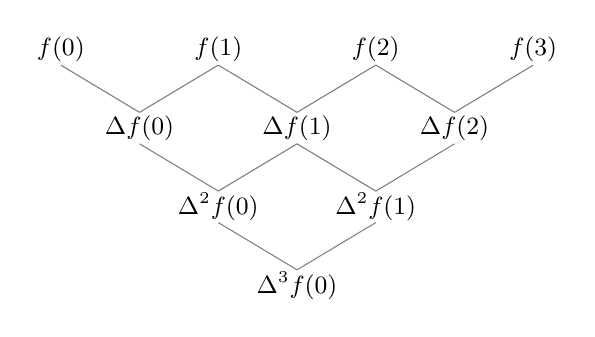
\begin{tikzpicture}[every node/.style={font=\small}]

\node at (0,0) {$f(0)$};
\node at (2,0) {$f(1)$};
\node at (4,0) {$f(2)$};
\node at (6,0) {$f(3)$};

\node at (1,-1) {$\Delta f(0)$};
\node at (3,-1) {$\Delta f(1)$};
\node at (5,-1) {$\Delta f(2)$};

\node at (2,-2) {$\Delta^2 f(0)$};
\node at (4,-2) {$\Delta^2 f(1)$};

\node at (3,-3) {$\Delta^3 f(0)$};

\draw[gray] (0,-0.2) -- (1,-0.8);
\draw[gray] (2,-0.2) -- (1,-0.8);

\draw[gray] (2,-0.2) -- (3,-0.8);
\draw[gray] (4,-0.2) -- (3,-0.8);

\draw[gray] (4,-0.2) -- (5,-0.8);
\draw[gray] (6,-0.2) -- (5,-0.8);

\draw[gray] (1,-1.2) -- (2,-1.8);
\draw[gray] (3,-1.2) -- (2,-1.8);

\draw[gray] (3,-1.2) -- (4,-1.8);
\draw[gray] (5,-1.2) -- (4,-1.8);

\draw[gray] (2,-2.2) -- (3,-2.8);
\draw[gray] (4,-2.2) -- (3,-2.8);

\end{tikzpicture}
\end{center}

The values along the left edge of the triangle determine the
coefficients in the Newton expansion.

\subsection*{Proof Sketch}

We construct the expansion term by term.

First observe that the constant function

\[
f(0)
\]

matches the value of \(f\) at \(x=0\).

Next, the function

\[
f(0) + \Delta f(0)\,x
\]

matches the values of \(f\) at \(x=0\) and \(x=1\).

Adding the term

\[
\frac{\Delta^2 f(0)}{2!}x^{\underline{2}}
\]

corrects the value at \(x=2\), while preserving the earlier values.
Continuing this process constructs a polynomial that agrees with \(f\)
at progressively more points.  The coefficients that accomplish this
are precisely the successive finite differences of \(f\).

\subsection*{Comparison with Taylor Series}

\begin{center}
\begin{tabular}{c|c}
\textbf{Continuous Calculus} & \textbf{Discrete Calculus} \\
\hline
Taylor series & Newton expansion \\
Derivative \(f^{(k)}(0)\) & Difference \(\Delta^k f(0)\) \\
Power \(x^k\) & Falling factorial \(x^{\underline{k}}\) \\
\end{tabular}
\end{center}

\begin{remark}
Just as Taylor series express smooth functions as combinations of
powers of \(x\), the Newton expansion expresses discrete functions as
combinations of falling factorials.  The coefficients are determined by
successive finite differences rather than derivatives.
\end{remark}


\begin{center}
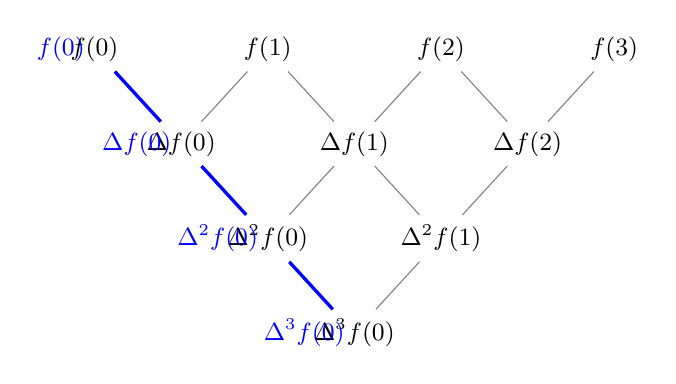
\begin{tikzpicture}[
every node/.style={font=\small},
x=2.2cm,
y=1.2cm
]

% top row
\node (f0) at (0,0) {$f(0)$};
\node (f1) at (1,0) {$f(1)$};
\node (f2) at (2,0) {$f(2)$};
\node (f3) at (3,0) {$f(3)$};

% first differences
\node (d0) at (0.5,-1) {$\Delta f(0)$};
\node (d1) at (1.5,-1) {$\Delta f(1)$};
\node (d2) at (2.5,-1) {$\Delta f(2)$};

% second differences
\node (d20) at (1,-2) {$\Delta^2 f(0)$};
\node (d21) at (2,-2) {$\Delta^2 f(1)$};

% third differences
\node (d30) at (1.5,-3) {$\Delta^3 f(0)$};

% connecting lines
\draw[gray] (f0) -- (d0);
\draw[gray] (f1) -- (d0);

\draw[gray] (f1) -- (d1);
\draw[gray] (f2) -- (d1);

\draw[gray] (f2) -- (d2);
\draw[gray] (f3) -- (d2);

\draw[gray] (d0) -- (d20);
\draw[gray] (d1) -- (d20);

\draw[gray] (d1) -- (d21);
\draw[gray] (d2) -- (d21);

\draw[gray] (d20) -- (d30);
\draw[gray] (d21) -- (d30);

% highlight left edge
\draw[very thick,blue] (f0) -- (d0) -- (d20) -- (d30);

\node[blue,left] at (f0) {$f(0)$};
\node[blue,left] at (d0) {$\Delta f(0)$};
\node[blue,left] at (d20) {$\Delta^2 f(0)$};
\node[blue,left] at (d30) {$\Delta^3 f(0)$};

\end{tikzpicture}
\end{center}


\begin{remark}
The coefficients in the Newton expansion are obtained from the left edge
of the difference table:

\[
f(0),\quad
\Delta f(0),\quad
\Delta^2 f(0),\quad
\Delta^3 f(0),\dots
\]

These values determine the expansion

\[
f(x)
=
f(0)
+
\Delta f(0)\,x
+
\frac{\Delta^2 f(0)}{2!}x^{\underline{2}}
+
\frac{\Delta^3 f(0)}{3!}x^{\underline{3}}
+\cdots .
\]

Each level of the difference table contributes one term in the
falling–factorial expansion.
\end{remark}


































